%!TEX root = ../../main.tex
\chapter{Dose Decay Modelling}
\label{chap:Dose Decay Modelling}

\section{Introduction}
\label{sec:Introduction - Dose Decay Modelling}

The diffraction weighted dose (DWD) is a dose metric that exhibits a consistent and reproducible relationship with the relative decay in total diffraction intensity from a protein crystal down to a relative intensity of 40\% \cite{zeldin2013dwd}.
This is because DWD spatially resolves the exposure of the crystal to the X-ray beam in addition to accounting for the absorbed dose.
Mathematically this spatial resolution of the exposure is incorporated via the fluence weighting in the DWD calculation (equation \ref{eq:DWD equation - no RDE}).
\textcolor{red}{
    \begin{myenumerate}
        \item \hypertarget{todo:include DWD equation again}{\textbf{TODO:} The \textbf{??} is a reference to the DWD equation}
        which is given in the introduction (it works when I include the whole thesis). Should I give the equation again here in this section?
    \end{myenumerate}
}
However, the DWD currently does not take into account the loss of diffraction ability due to the current damage state of the crystal.
The \textit{relatitive diffraction efficiency (RDE)}, $\eta$, is introduced as a function of the absorbed dose that describes the diffracting ability of any given volume of the crystal.
The RDE is defined as the ratio of the proportion of incident photons that are currently being diffracted to the proportion that initially diffracted.
This is graphically depicted in Figure~\ref{fig: Graphical depiction of RDE}.
\begin{figure}
        \centering
        \begin{subfigure}[b]{1\textwidth}
                \centering
                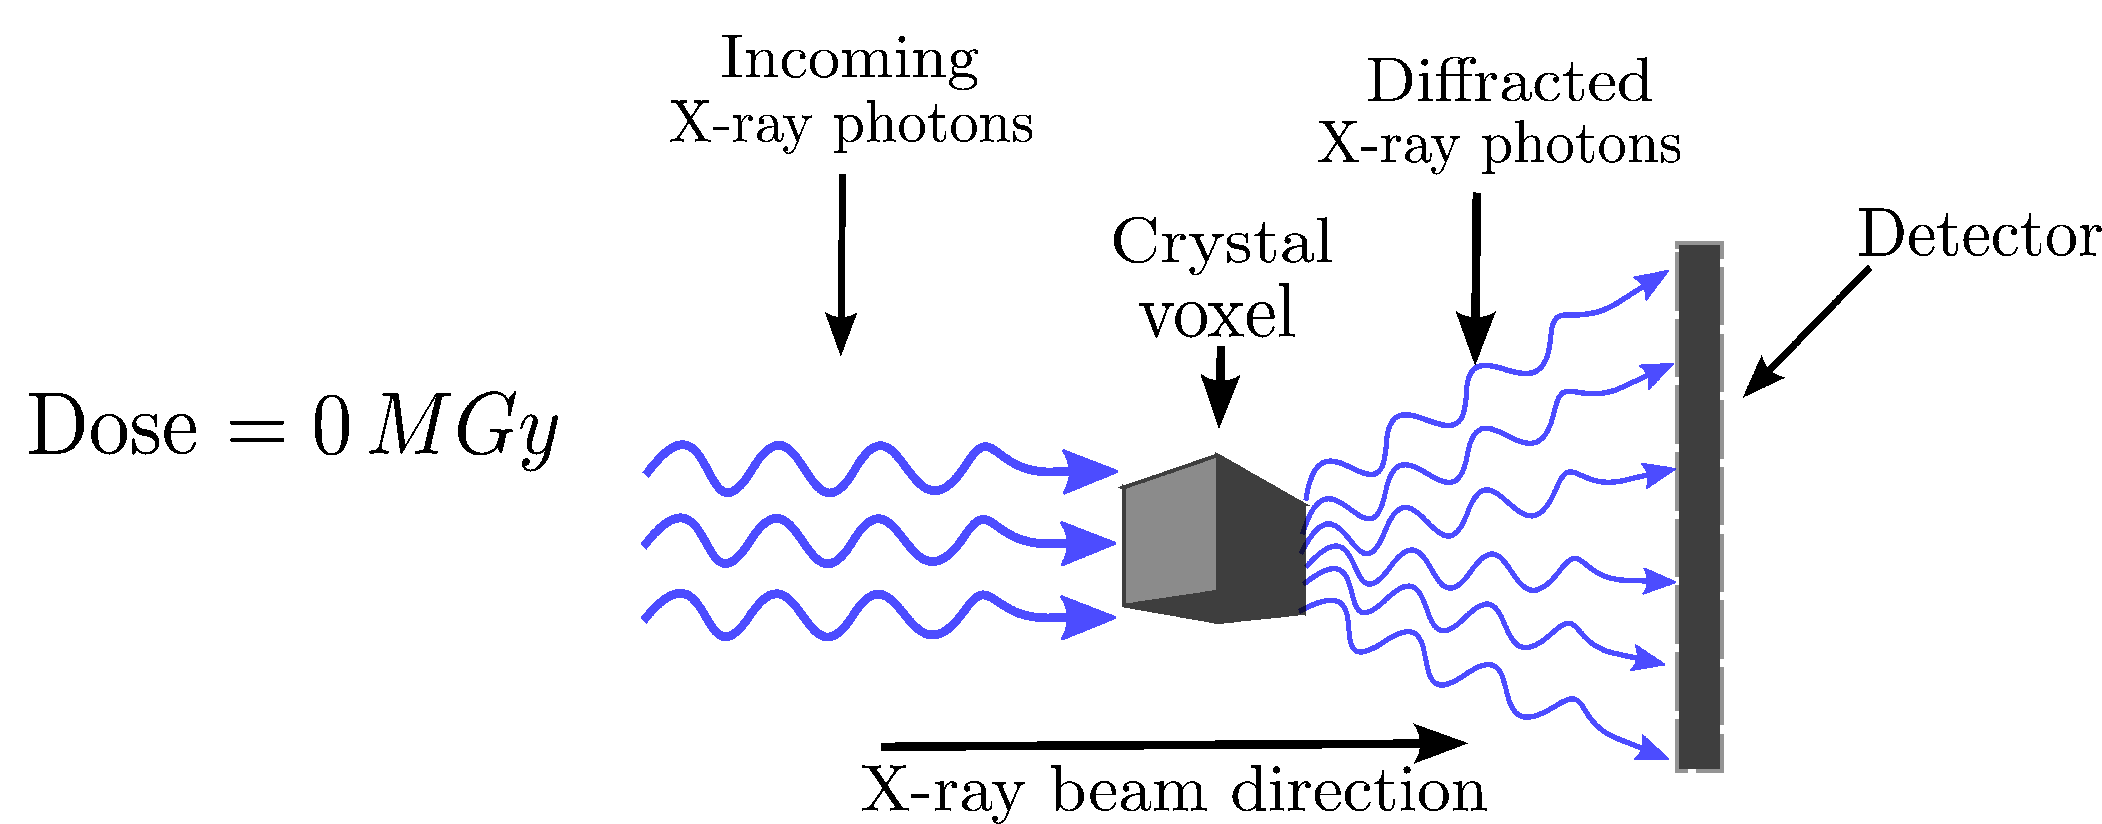
\includegraphics[width=\textwidth]{figures/dwd/rde1.pdf}
                \caption{}
                \label{fig:Graphical depiction of RDE - 0 MGy}
        \end{subfigure}
				\\
        \begin{subfigure}[b]{1\textwidth}
                \centering
                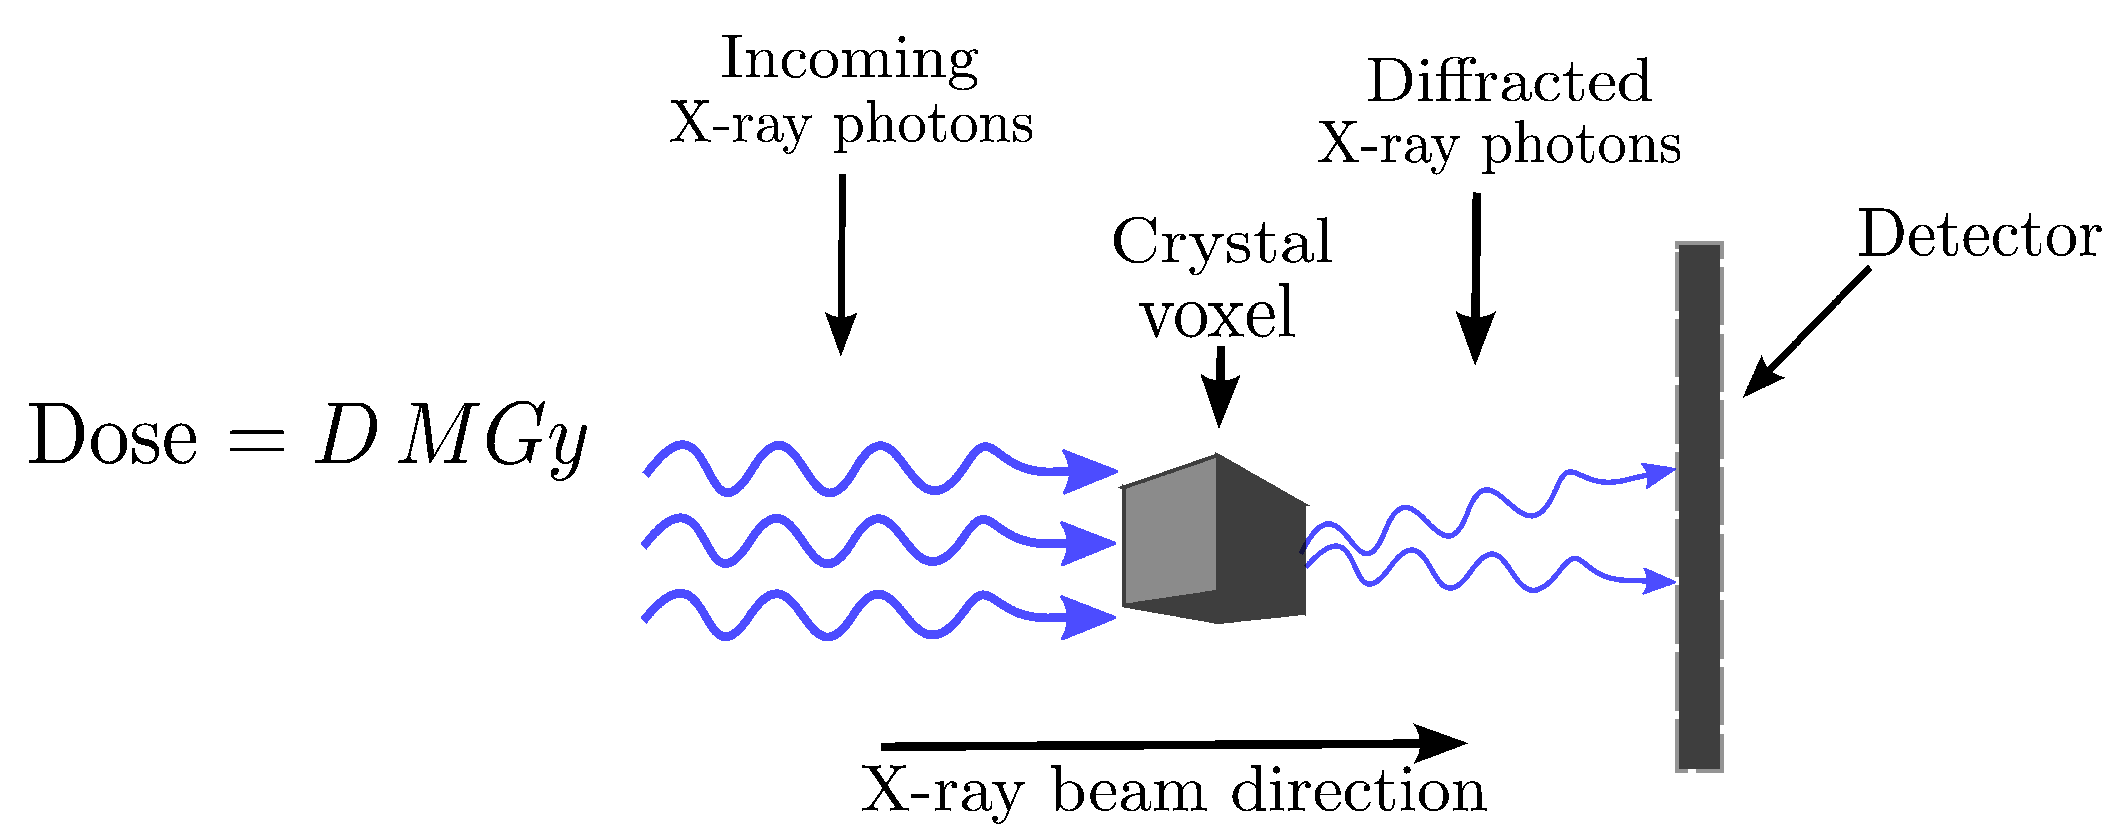
\includegraphics[width=\textwidth]{figures/dwd/rde2.pdf}
                \caption{}
                \label{fig:Graphical depiction of RDE - D MGy}
        \end{subfigure}
        \caption{A visual example of the relative diffraction efficiency (RDE).
        (a) Initially at dose = $0\, MGy$ the crystal voxel elastically scatters 6 photons for a given number of incident photons.
        (b) Later in the experiment when the crystal voxel has absorbed a dose $= D\, MGy$, it elastically scatters only 2 photons for the same number of incident photons.
        The ratio of the current number of diffracted photons with the initial number is $2/6 = 1/3$, therefore in this example the RDE is 1/3.}
        \label{fig: Graphical depiction of RDE}
\end{figure}

The RDE is incorporated into the DWD equation as additional weighting term.
Explicitly this is
\begin{equation}
    DWD^i = \f{\int_{t_{i-1}}^{t_{i}} \iiint_{crystal} D(\bs{x},t) \times F(\bs{x},t) \times \eta(D(\bs{x},t)) \quad \mathrm{d}\bs{x}\mathrm{d} t}{\int_{t_{i-1}}^{t_{i}} \iiint_{crystal}F(\bs{x},t) \times \eta(D(\bs{x},t)) \quad \mathrm{d}\bs{x}\mathrm{d} t}.
    \label{eq:DWD equation with RDE}
\end{equation}

The work presented in this chapter describes the experiment and analysis carried out to determine a suitable functional form for the RDE.
Finally the RDE is then incorporated to the DWD using equation \ref{eq:DWD equation with RDE} and compared to the simple DWD (equation \ref{eq:DWD equation - no RDE}) with the data used in the previous DWD study \cite{zeldin2013dwd}.
